%************************************************
\chapter{Methods}
\label{chp:Meth}
%************************************************

\section{Digital aerial photogrammetry}\label{sec:DAP}

\subsection{General Considerations on Image Matching}

Photogrammetry\index{photogrammetry} \graffito{3d coordinates of objects can be derived from stereo images via photogrammetry.} is a measurement technique
to derive 3d\index{three-dimensional} coordinates of object points, which are depicted on 
images taken from different positions \parencite{Lemmens.2011b}.
By utilizing the stereophotogrammetric measuring principle (see subsection~\ref{subsec:HeighAssessStereo}) 
and with known orientation\index{image orientation} parameters of the images\footnote{\emph{interior orientation:}\index{image orientation!interior orientation} 
	focal length, principal point ($X, Y$), pixel size;
	\emph{exterior orientation:}\index{image orientation!exterior orientation} position coordinates of the projection centre ($X, Y, Z$), 
	plus angular parameters ($\omega, \phi, \kappa$).},
 the coordinates of the objects of interest can be retrieved via triangulation\index{triangulation}.
According to \textcite[p. 231]{Schenk.1999}, 

\begin{quote}
”[o]ne \graffito{Identification and measurement of conjugate points in overlapping images is fundamental in photogrammetry.}
of the most fundamental processes in photogrammetry
is to identify and to measure conjugate
points in two or more overlapping photographs.
Stereo photogrammetry relies entirely on conjugate
points. In analogue and analytical photogrammetry
the identification of conjugate points
is performed by a human operator; in digital photogrammetry
one attempts to solve the problem
automatically -- a process known as image matching\index{image matching}.”
\end{quote}

\noindent The introduction of stereo-image matching techniques in photogrammetry allowed for automation in different processing steps, 
particularly in the creation of dense height measurements, and is the fundamental basis for \ac{DAP}.
Generally speaking, the aim of image matching is to identify corresponding pattern in the stereo-image pairs, 
\ie, the base and the match image. The problem in finding these correspondences is to trace and locate the pattern 
in the match image as the conjugate of a pattern in the base image \parencite{Lemmens.2011b}.

Traditionally, the image-matching methods \graffito{Established image matching categories: \emph{feature-based} and \emph{area-based} matching.}
may be assigned to two categories depending
on how the image -- an array of pixels storing digital numbers -- is approached \parencite{ERDAS.2010, Gruen.2012}.
The first category can be classified as \emph{feature-based matching} approaches\index{image matching!feature-based matching}. 
These focus on the evaluation of similarities 
of extracted features in both base and match image, which may be depictions of prominent features like corners of buildings, road crossings,
or solitaire trees in case of aerial photographs.
The second group of algorithms can be categorized as \emph{area-based matching} approaches\index{image matching!area-base matching}.
Here, correspondence between the stereo images is sought using the grey level values in regularly shaped patches, \eg, 9\,x\,9\,pixel windows. 
A reference window, remaining at a constant location in the base image, is defined as source for calculating correlation to 
candidate windows on the match image. Many different search windows in the match image are evaluated until the location for correspondence is
determined by the highest value for the correlation coefficient. 
Consequently, the centre pixels of the reference and search window are selected as corresponding points.
Most commonly, normalized cross-correlation (NCC)\index{normalized cross-correlation} is used for calculating correlation and acceptance of the match 
depends on whether the similarity value exceeds a predefined threshold \parencite{Lemmens.2011b}. 
A trade-off is associated with the definition of the correlation threshold: whereas choosing too small values allows for many mismatches, \ie,
wrong correspondences of pixels, too high values impede many matches and in consequence, the density of matches found for a stereo-image pair decreases.

\subsection{Semi-global Matching}\index{semi-global matching}

Problems with finding correspondences are especially connected to object boundaries, fine structures, low and repetitive textures, and recording
and illumination differences in the images.
In order to overcome these drawbacks, effort was put into developing new image-matching methods.
One approach which have gained considerable attention in recent years, is the so-called \acf{SGM} technique\index{SGM|see{semi-global matching}} introduced by \textcite{Hirschmuller.2005,Hirschmuller.2008}.
\ac{SGM} is based on the idea of pixelwise matching\index{image matching!pixelwise matching} and approximating a global 2d smoothness constraint by combining 
many 1d constraints.
The basic steps of \ac{SGM} are:
\begin{itemize}
	\item Generation of epipolar images\index{epipolar images} by projectively warp the base and match images with known geometries 
		such that the epipolar lines are horizontal.
	\item Calculation of possible disparities\index{disparity} for each pixel along the epipolar search lines in the base image and computation of 
		matching costs\index{matching cost} for each candidate disparity by a similarity measure (\eg, Mutual Information, Census) comparing the pixel grey values. 
	\item Aggregation of costs by pathwise accumulation of minimal costs along a certain number of 1d path directions through the base image.
		Here, additional smoothness constraints are introduced by penalizing disparity changes.
	\item Determination of final disparities for each pixel in the base image by selecting the candidate pixel in the match image 
		that corresponds to the minimum cost.
	\item Intersection of viewing rays in the stereo images according to the final disparity image to achieve 
	dense 3d\index{three-dimensional} point clouds\index{point cloud} in object space. 
\end{itemize}
More details regarding the performed steps in \ac{SGM} and the implemented algorithms are provided in, \eg, \textcite{Hirschmuller.2008,Hirschmuller.2011} and \textcite{Gehrke.2010}.

We applied the \ac{SGM} approach for image matching\index{image matching} and consecutive derivation of image-based surface heights throughout the studies
presented in this work\footnote{except for \textcite{Immitzer.2016}: here, the area-based normalized cross-correlation method implemented 
	in LPS eATE (ERDAS IMAGINE 2014) was used.}. 
For the processing, we used the \ac{SGM} implementation within the Remote Sensing Software Package Graz (RSG).
The cost function used in RSG follows the Census disparity measure, and 
the matching procedure is hierarchically structured as coarse to fine matching, with consequent disparity calculations on four image pyramid levels. 

We selected the panchromatic\index{panchromatic} band \graffito{Panchromatic images were used for matching of along-track stereo-image pairs covering the Bavarian test sites.}
of the stereo images for matching in all Bavarian test sites. Due to the low across-track overlaps of the images,
we used only stereo-image pairs from the along-track overlap for calculation.
For the \ac{NVI} test site, the airphotos were only available as multispectal\index{multispectral} images (\emph{RGBI}). Here, the green band was selected for matching.

As outputs from dense stereo matching in RSG, we opted for using the raw dense 3d point clouds from the respective stereo pairs and used additional utility software for 
further processing. In the work concerned with the assessment of height changes \parencite{Stepper.2015}, 
we used \acp{DSM}\index{digital surface model}\index{DSM|see{digital surface model}} as outputs from the RSG streamline for further analysis.
  
The products from \ac{DAP}, \ie, the dense image-based point clouds or the \acp{DSM}, were further processed to calculate the object heights above ground 
by using the \ac{ALS}-based elevation heights for subtraction. 
Subsequently, different data processing steps (clipping to inventory point geometries, etc.) were performed in order to prepare appropriate data sets for 
consequent use in statistical modelling. Details regarding the particular processing steps are given in the respective paper sections.
 

\section{Statistical Modelling}\label{sec:StatModel}

As introduced in sections~\ref{sec:AerialPhotogrammetry} and~\ref{sec:ABA},
the \acf{ABA} gained strong interest for integrating remote sensing data sets, in particular \ac{ALS} and \ac{DAP}-based products,
for use in forest inventory and mapping applications.

% long sentence, maybe split into two shorter!
In this context, \ie, for the combination of ground based measurements and the remotely sensed data, statistical models which can produce
unbiased and accurate estimates of the forest attribute\index{forest inventory attribute} of interest by means of remote sensing predictor variables\index{predictor variable}
play a key role. 
In the \ac{ABA}\index{area-based aproach} workflow (see Figure~\ref{fig:ABA_method}), the statistical models are trained with known samples, 
namely the ground-based inventory measurements and the descriptive statistics (\mbox{\emph{metrics}}) calculated 
from the remote sensing data clipped to the areas of the georeferenced inventory plots --
and consequently, these models are applied to predict estimates over entire forest areas.

Therefore \graffito{The statistical model describes the dependency between the remote sensing predictors and the ground-based response.}
it is crucial, that the chosen model type is able to accurately map the statistical dependency between the remote sensing predictor variables
and the response variables\index{response variable} derived from the ground measurements (\eg, mean stand height or volume).
In the literature, different regression\index{regression model} approaches (parametric\index{regression model!parametric} 
and non-parametric\index{regression model!non-parametric}) were applied to fulfil this task. 
Besides linear regression modelling, the decision-tree based approach \acf{RF}\index{regression model!non-parametric!random forest} 
was most widely used for predictive modelling of 
forest inventory attributes through the course of the presented studies.
Therefore, and without judging other approaches for their appropriateness, the main characteristics of \ac{RF} and its actual application are described.

\subsection{Random Forest for Regression}

\ac{RF} can be assigned to \graffito{\ac{RF} requires no a priori assumption about the relationship of predictors and response variables.}
the domain of non-parametric modelling approaches.
Thus, no \emph{a priori} assumptions about relationships between predictor\index{predictor variable} and response variables\index{response variable} 
are made \parencite{White.2013}.
Due to that, and to the fact that very little tuning is required during model building, \ac{RF} has become a popular method in predictive modelling.

\ac{RF}, developed by \textcite{Breiman.2001}, is an ensemble regression tree algorithm (see Algorithm~\ref{algo:RF}) based on a 
large collection of \emph{de-correlated} decision trees\index{regression model!non-parametric!decision tree} \parencite{Hastie.2009}. 
\ac{RF} \graffito{An ensemble of de-correlated decision trees forms a \ac{RF} model.}
can be seen as further development of bagging (\emph{bootstrap aggregation}), as the individual trees that constitute the forest are 
fitted to bootstrap-sampled versions of the training data, and averaged to get the final result
(for a schematic of \emph{bootstrap sampling}, see Figure~\ref{fig:bootstrap}).

In \ac{RF}, a second randomization is introduced to the tree-building process, in order to additionally reduce the correlation between the trees: 
the algorithm randomly selects a subset of predictor variables as candidates for splitting at each decision node.
\ac{RF} has two potential parameters for adjustment: 
(a)~the number of randomly selected predictors \emph{m}, from which to choose at each split 
(commonly referred to as $m_{\textsf{try}}$). 
For use in regression, the algorithm inventor \citeauthor{Breiman.2001} recommended $p/3$ as default value, \ie, one third of the 
number of predictors \parencite{Breiman.2001}; (b) the number of trees in the forest (commonly referred to as $n_{\textsf{tree}}$). 
As \ac{RF} is not prone to over-fitting, large numbers of trees do not adversely affect the model accuracy. 
However, the computational expense increases. \textcite{Kuhn.2013b} suggest 1\,000 trees as starting point,
and adjustment in dependence of the achieved model performance.
Important advances and features of \ac{RF} are:

\begin{description}
	\item[distribution independence] The variables ($x, y$) used as predictors and response in modelling do not have to follow a predefined distribution.
	\item[dimensionality] In \ac{RF}, high-dimensional and highly correlated data sets can be processed without suffering a loss in performance.
	\item[\acf{oob}]\index{out-of-bag} For each observation $z_i = (x_i, y_i)$, its random forest predictor can be computed by averaging only those trees corresponding to 
		bootstrap samples in which $z_i$ is not included (see Figure~\ref{fig:bootstrap}). 
		Doing so, an \ac{oob} error estimate is almost identical to that obtained by
		N-fold cross-validation (cf. \cite{Hastie.2009}). 
		Thus, performance measures can be computed along the way during \ac{RF} model training.
	\item[variable importance] Information on the importance of each predictor variable used in model building can be computed twofold: 
		(a) as measure of the total decrease in node impurities from splitting on each variable, averaged over all trees; 
		(b) as mean decrease of prediction accuracy, when permuting the values of the predictor variables in the \ac{oob} samples, again averaged over all trees. 
\end{description}



\begin{figure}[tb]
	\centering
	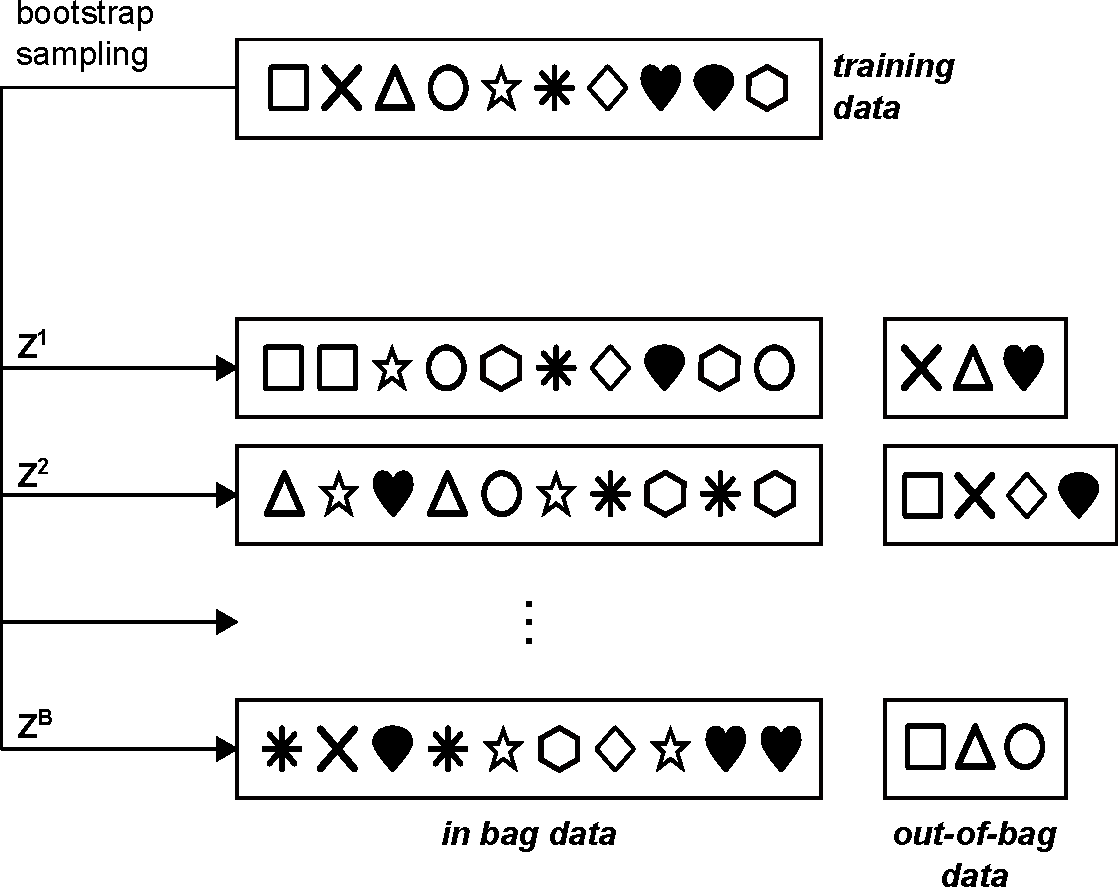
\includegraphics[width=.8\textwidth]{Figures/bootstrap/bagging_RF_landscape} %scale for golden ratio 0.618
	\caption[Schematic of bootstrap resampling used in Random Forests.]
	{Schematic of bootstrap resampling as used in \ac{RF} for drawing the training samples for the individual regression trees.
		The training sample data are depicted as symbols and are allocated to \emph{B} subsets, each taken as random sample \emph{with replacement}.
		The subsets are of the same size as the original training data and can contain multiple instances of the same data point. Samples not selected by the
		bootstrap\index{bootstrap} are the \emph{out-of-bag}\index{out-of-bag} data and can be used to estimate model performance (modified after \cite{Kuhn.2013b}).}
	\label{fig:bootstrap}
\end{figure}



\begin{algorithm}[bt]
	\SetAlCapFnt{\small\sffamily\bfseries}
	\SetAlCapNameFnt{\small}
	\small
	%\TitleOfAlgo{test}
	%\SetAlgoLined
	\DontPrintSemicolon
	
	Select the number of trees to build, \emph{B}:\;
	\BlankLine
	\For{b = 1 to B:}{
		(1) Draw a bootstrap sample \textbf{Z*} of size \emph{N} from the training data.\;
		(2) Train a tree model $T_b$ to the bootstrapped data, by recursively repeating the following steps for each terminal node of the tree,
		until the minimum node size $n_{\textsf{min}}$ is reached.\;
		\For{each split:}{
			(a)\:Select \emph{m} variables at random from the \emph{p} predictor variables (\emph{m}\,$\leq$\,\emph{p}).\;
			(b)\:Pick the best variable/split-point among the \emph{m}.\;
			(c)\:Split the node into two data nodes.
		}
	}
	\BlankLine
	Output the ensemble of trees $\left\lbrace T_b\right\rbrace _1^B$.\;
	\BlankLine
	To make a prediction at a new point \emph{x}:\;
	$\hat{f}_{rf}^B(x)=\frac{1}{B}\sum_{b=1}^B T_b(x)$
	
	\caption{Random Forest for Regression (modified after \cite{Hastie.2009} and \cite{Kuhn.2013b}).}
	\label{algo:RF}		
\end{algorithm}


\subsection{Model Implementation for predicting Forest Inventory Attributes}\index{forest inventory attribute}

We used functionalities and add-on packages of the open-source statistical software \textsf{R} to accomplish all statistical tasks.
For model development (using the data gathered at the forest inventory plots) and prediction to unknown samples by means of \ac{RF},
the functionalities provided in the packages \textsf{caret} \parencite{Kuhn.2015} and \textsf{randomForest} \parencite{Liaw.2002} were principally used. 
 
With regard to the tuning parameters of \ac{RF}\index{random forest}, we followed the recommendation of \textcite{Kuhn.2013b}: 
The number of regression trees in the respective forests was set to $n_{\textsf{tree}} = 1000$, 
and the number of variables randomly selected at each split was set to $m_{\textsf{try}} = p/3$.

In all studies, the \acf{RMSE}\index{RMSE|see{root mean squared error}}\index{root mean squared error} and 
\acf{ME}\index{ME|see{mean error}}\index{mean error} measures were selected to evaluate model performance, \ie, model accuracy\index{accuracy} and bias\index{bias}.
In the studies of \textcite{Stepper.2015b,White.2015,Straub.2016}, we applied a 10-fold cross-validation\index{cross-validation} repeated five times to assess model performance
and in the studies of \textcite{Immitzer.2016,Stepper.2016} the \ac{oob}-estimates\index{out-of-bag} were used for model evaluation.

Additionally, the model performance at the stand level, \ie, after wall-to-wall prediction mapping and aggregating to forest stands, 
was examined in the studies of \textcite{Stepper.2015b, Immitzer.2016}.
Independent inventory data from nearby forests were utilized to assess model transferability in the study of \textcite{Stepper.2016}, 
again by means of \ac{RMSE} and \ac{ME}.
For more details regarding model training and evaluation, the reader is referred to the respective articles. 


\section{Height Change Assessment}\label{sec:HeightChange}

Elaborating on the aim to test the utility of digital stereo images from repeat surveys for forest height change assessment,
we developed a workflow as illustrated in Figure~\ref{fig:meth_heightChange}.

\begin{figure}[!b]
	\centering
	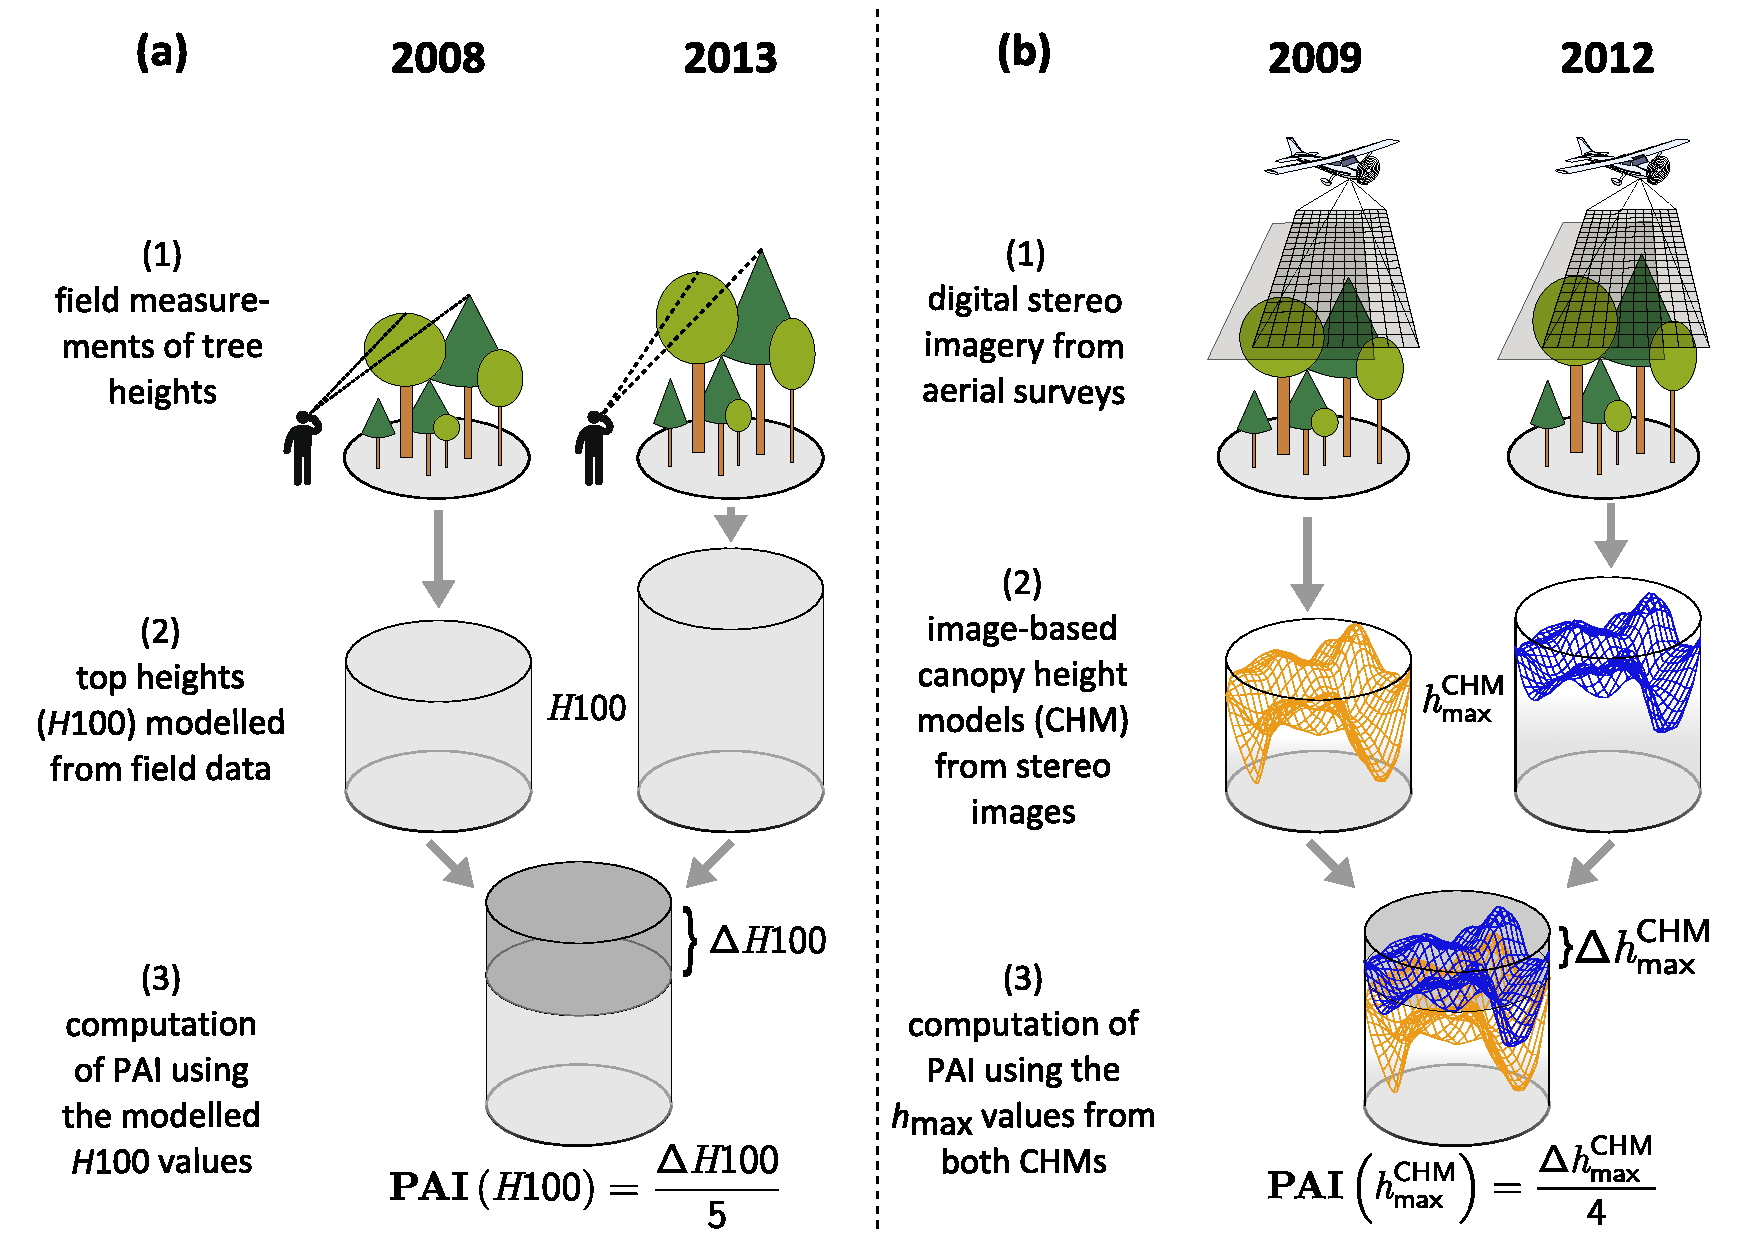
\includegraphics[width=1\textwidth]{Figures/heightChange/Method_heightChange} %scale for golden ratio 0.618
	\caption[Methodological workflow for height change assessment using terrestrial measurements and image-based CHMs.]
	{Methodological workflow for height change assessment using terrestrial measurements and \acp{CHM}\index{canopy height model}\index{CHM|see{canopy height model}} 
		based on stereo airphotos from repeat aerial image surveys. \textbf{(a)} Terrestrial assessment: 
		(1) tree crown heights are measured for representative samples at the respective inventory plots, 
		(2) top heights ($H100$) are modelled using the height measurements of trees from the overstory and emergent tree layers, 
		(3) \ac{PAI}\index{periodic annual increment}\index{PAI|see{periodic annual increment}} is calculated as the difference between 
		the modelled $H100$ values for
		the two inventory dates divided by the time lapse between the two inventories. 
		\textbf{(b)} Aerial image assessment: 
		(1) digital stereo images are acquired in regularly scheduled aerial surveys, 
		(2) \acp{CHM} are created by subtracting \ac{LiDAR}-derived terrain heights from image-based surface models, 
		(3) \ac{PAI} is computed as the difference between the maximum height
		values ($h_{max}$) from the two \acp{CHM} divided by the time lapse between the two image dates.}
	\label{fig:meth_heightChange}
\end{figure}

We followed the \ac{SGM}\index{semi-global matching} approach (see section~\ref{sec:DAP}) to accomplish image matching\index{image matching} of the stereo airphotos. 
In our study \parencite{Stepper.2015},
we chose the RSG software utilities for image matching and used the implemented functionality to output \acp{DSM} with 1\,m resolution for both dates of image acquisition.
Finally, \acp{CHM} were derived by subtracting the elevation values of the bare earth \ac{DTM} from the z-values of the two \acp{DSM}.

Terrestrial inventory measurements, acquired for circular 500\,m\textsuperscript{2} plots, 
were used as reference for the assessment of forest canopy height and height changes.
$H100$ was calculated from the field measurements as height metric approximating top heights of forest stands. In our study, $H100$ was 
defined as the average height of the 100 stems per hectare with the largest \acp{DBH} (see \emph{Algorithm~1} in the article for the explicit computation rule set). 

To link the \ac{CHM}-heights with the field-based $H100$ top heights, various height percentiles (25th, 50th, 75th, 90th, 95th, and maximum) were calculated
from the \ac{CHM}-values for the areas within each of the 500\,m\textsuperscript{2} circular plots.
The percentiles\index{percentile} were correlated to the field-based top heights and 
the maximum height of the \ac{CHM} ($h_{max}$) turned out to achieve highest correlation values.
Thus, this variable was selected for the height change assessment.

Height differences between the two points in time from the terrestrial and the aerial image acquisitions were used to calculate \acfp{PAI} as 
standardized increment measures per unit of time (see Figure~\ref{fig:meth_heightChange}).
The \acp{PAI}, both from the field measurements and the image-based height data, were regressed against the $H100$ top height values based on the 
initial field data (from $t_{1,\textsf{field}}$) to analyse the relationship between initial forest height and height growth.
Finally, differences between increments for initial height classes representing various forest successional stages were examined.  


